\documentclass[aspectratio=1610]{beamer}
\usepackage[utf8]{inputenc}
\usepackage[T1]{fontenc}
\usepackage[german]{babel}
\usepackage[useregional]{datetime2}
\usepackage[nameinlink]{cleveref}
\usepackage[section]{placeins}
\usepackage{xcolor}
\usepackage{graphicx}
\usepackage{csquotes}
\usepackage{amsmath} % for $\text{}$
\usepackage{enumitem}
\setlist{nosep}


\newcommand\urlpart[2]{$\underbrace{\text{\texttt{#1}}}{\text{#2}}$}
\raggedbottom
\crefname{figure}{Abb}{Abb}

\newcommand\producttitle{treff.}
\hypersetup{
	pdftitle={Implementierung: \producttitle},
	bookmarks=true,
}


% header & footer
\usepackage{scrlayer-scrpage}
%\lofoot{\today}
%\refoot{\today}
\pagestyle{scrheadings}

\title{
\includegraphics[width = 50mm]{images/logo_crop.png}}
\subtitle{\huge Implementierung}
\author{Lukas Dippon
	\and Jens Kienle
	\and Matthias Noll
	\and Fabian Röpke
	\and Tim Schmidt
	\and Simon Vögele}

\begin{document}

	\begin{frame}[plain]
	\maketitle
	\end{frame}

%%%%%%%%%%%%%%%%%%%%%%%%%%%%%%%%%%%%%%%%%%%%%%%%%%%%%%%%%%%%%%%%%%%%%
%%%% Entwurf
%%%%%%%%%%%%%%%%%%%%%%%%%%%%%%%%%%%%%%%%%%%%%%%%%%%%%%%%%%%%%%%%%%%%%

	\begin{frame}[plain]
		\frametitle{Entwurf}

		\begin{minipage}{0.5\textwidth}
		placeholder (image)
		\end{minipage}%
		\begin{minipage}{0.5\textwidth}
		\textbf{Freundschaftsanfragen}
		\begin{itemize}
			\setlength\itemsep{0.3em}
            \item[--] Verhindern ungewollte Massen-Gruppenhinzufügungen durch
                einen Nutzer
            \item[--] Dämmen Spam durch viele Nutzer
                \begin{itemize}
                    \item[--] \enquote{Alle Kontaktanfragen ablehnen} hat
                        weniger gravierende Nebeneffekte als \enquote{Alle
                        Gruppen verlassen}.
                \end{itemize}
		\end{itemize}
		\end{minipage}

	\end{frame}

%%%%%%%%%%%%%%%%%%%%%%%%%%%%%%%%%%%%%%%%%%%%%%%%%%%%%%%%%%%%%%%%%%%%%
%%%% Klient
%%%%%%%%%%%%%%%%%%%%%%%%%%%%%%%%%%%%%%%%%%%%%%%%%%%%%%%%%%%%%%%%%%%%%

	\begin{frame}[plain]
		\frametitle{Klient - State}
		\textbf{Funktionsweise}
		\begin{itemize}
			\setlength\itemsep{0.3em}
			\item[--] \textbf{class State:} Wrapper für ViewCall und int
			\item[--] \textbf{enum ViewCall:} mögliche Anfragen an Context
			\item[--] \textbf{SingleLiveEvent:} Observable, wartet auf
			genau einen Listener
			\item[--] \textbf{in ViewModel:} setValue des state
			\item[--] \textbf{in Activity:} observe des state um UI-Aufrufe
			zu starten
		\end{itemize}
	$\Rightarrow$ verhindert Aufrufe auf gelöschte Views \\
	$\Rightarrow$ verhindert starke Kopplung zwischen ViewModel und View
	\end{frame}

	\begin{frame}[plain]
	\frametitle{Klient - RequestEncoder}
	\textbf{Fassade für Commands}
	\begin{itemize}
		\setlength\itemsep{0.3em}
		\item[--] Entkopplung der Commands
		\item[--] Einheitliches Verhalten
		\item[--] werden als Queue abgearbeitet
 	\end{itemize}
	\end{frame}

	\begin{frame}[plain]
	\frametitle{Klient - Commands}
	\begin{itemize}
		\setlength\itemsep{0.3em}
		\item[--] Halten innere Klassen, die den JSON Objekten der Befehle entsprechen
		\item[--] Serialisierung durch Jackson Library
		\item[--] Verarbeiten Serverantworten (Einpflegen in Datenbank o.Ä.)
 	\end{itemize}
	\end{frame}

	\begin{frame}[plain]
	\frametitle{Klient - Commands}
	\begin{figure}[h]
		\centering
		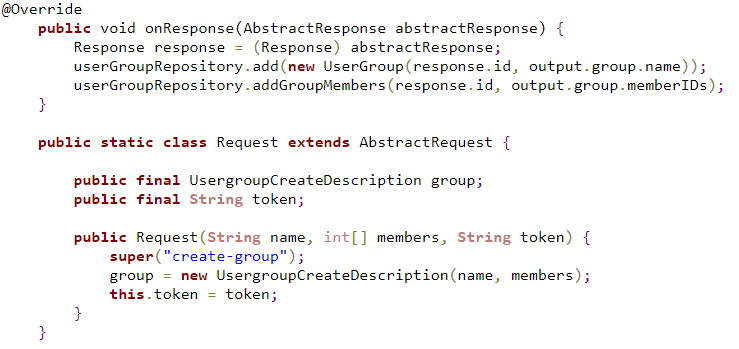
\includegraphics[width=0.8\textwidth]{images/CreateGroupCommand.PNG}
		\caption{Beispiel mit Request Klasse und onResponse Methode}
	\end{figure}
	\end{frame}

	\begin{frame}[plain]
	\frametitle{Klient - Repositories}
	\begin{figure}[h]
		\centering
		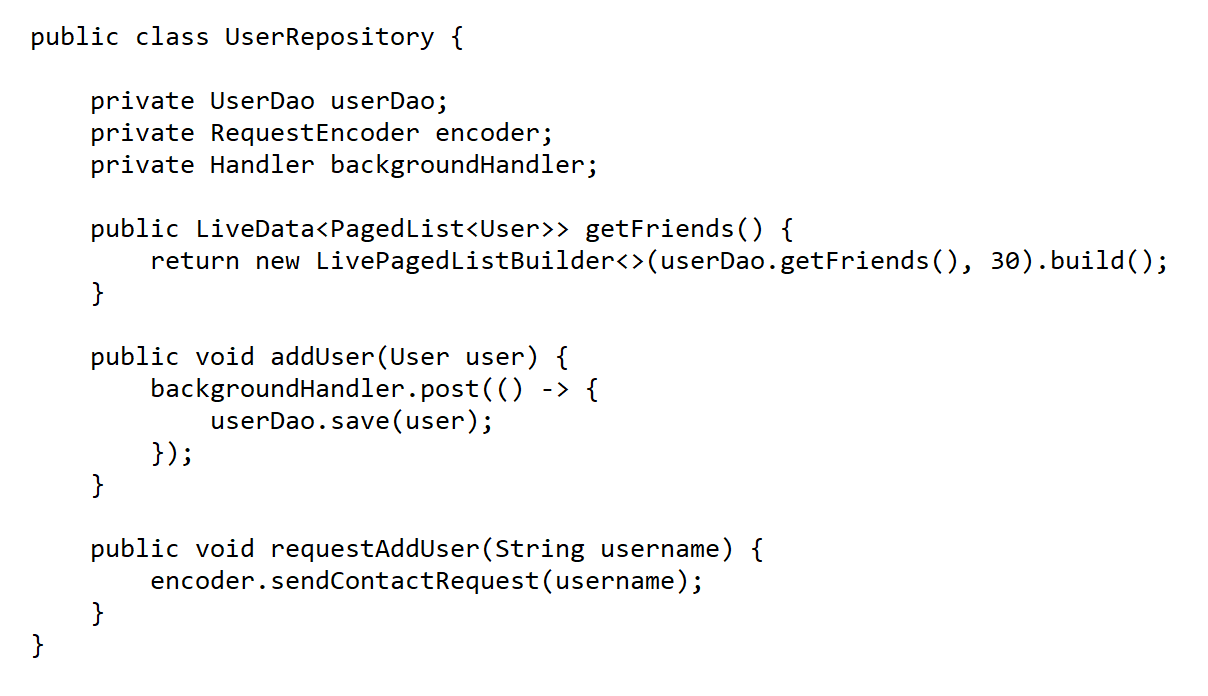
\includegraphics[width=0.8\textwidth]{images/UserRepository.PNG}
		\caption{getrennte Methoden für ViewModels und Encoder}
	\end{figure}
	\end{frame}

	\begin{frame}[plain]
	\frametitle{Klient - ViewModelFactory}
	\begin{figure}[h]
		\centering
		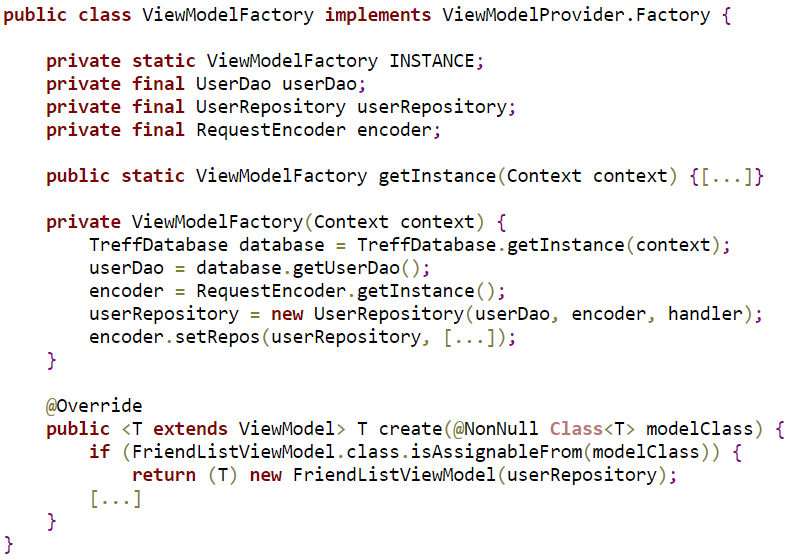
\includegraphics[width=0.8\textwidth]{images/ViewModelFactory.png}
		\caption{Erstellen aller ViewModels}
	\end{figure}
	\end{frame}

	\begin{frame}[plain]
	\frametitle{Klient - Karte}
	\begin{figure}[h]
		\centering
		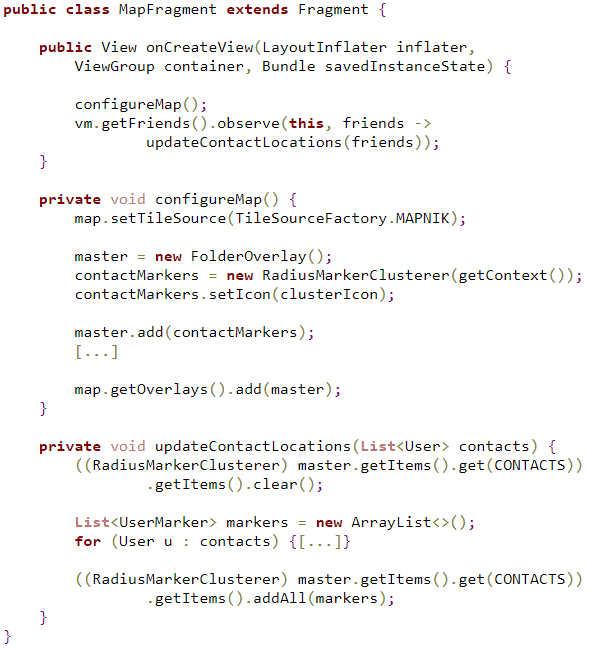
\includegraphics[width=0.5\textwidth]{images/MapFragment.png}
		\caption{Clustering und Positionsupdates der User}
	\end{figure}
	\end{frame}


%%%%%%%%%%%%%%%%%%%%%%%%%%%%%%%%%%%%%%%%%%%%%%%%%%%%%%%%%%%%%%%%%%%%%
%%%% SERVER
%%%%%%%%%%%%%%%%%%%%%%%%%%%%%%%%%%%%%%%%%%%%%%%%%%%%%%%%%%%%%%%%%%%%%

	\begin{frame}[plain]
		\frametitle{Server - Commands}
        \begin{figure}[h]
            \centering
            \includegraphics[width=0.6\textwidth]%
            {build/uml/server-request-journey.png}
            \caption{Ablauf der Anfragenbearbeitung}
        \end{figure}
	\end{frame}

	\begin{frame}[plain]
		\frametitle{Server - Command I/O}
        \begin{figure}[h]
            \centering
            \includegraphics[width=1\textwidth]%
            {images/server-io.png}
            \caption{Commands definieren ihren Input und Output}
        \end{figure}
	\end{frame}

	\begin{frame}[plain]
        \frametitle{Server - Deserialisierung in einfache POJOs}
        \begin{figure}[h]
            \centering
            \includegraphics[width=1\textwidth]%
            {images/server-usergroup-create-description.png}
            \caption{Alle für create-group verlangte Gruppenattribute}
        \end{figure}
	\end{frame}

	\begin{frame}[plain]
        \frametitle{Server - Serialisierung mittels eigener Serializer}
        \begin{figure}[h]
            \centering
            \includegraphics[width=1\textwidth]%
            {images/server-usergroup-serializer.png}
            \caption{Serializer fürs serialisieren von Gruppen in vollständige
            Beschreibungen}
        \end{figure}
	\end{frame}

	\begin{frame}[plain]
        \frametitle{Server - Gemeinsame Vorbereitungsschritte in abstrakter
        Überklasse}
        \begin{figure}[h]
            \centering
            \includegraphics[width=0.9\textwidth]%
            {images/server-abstract-command.png}
            \caption{Command-Klassen erben von AbstractCommand}
        \end{figure}
	\end{frame}

	\begin{frame}[plain]
		\frametitle{Server - Auswechselbares Backend}
        \begin{figure}[h]
            \centering
            \includegraphics[width=1\textwidth]%
            {images/server-interfaces-sql.png}
            \caption{Interfaces und SQL-Implementierungen für Objekte des
            semantischen Datenmodells}
        \end{figure}
        \begin{figure}[h]
            \centering
            \includegraphics[width=1\textwidth]%
            {images/server-choice.png}
            \caption{Wahl der SQL-Implementierung}
        \end{figure}
	\end{frame}

	\begin{frame}[plain]
		\frametitle{Server - SQL-Implementierung}
        \begin{figure}[h]
            \centering
            \includegraphics[width=1\textwidth]%
            {images/server-get-all-groups.png}
            \caption{Methoden der SQL-Klassen sind read-/write-through}
        \end{figure}
        \begin{figure}[h]
            \centering
            \includegraphics[width=0.8\textwidth]%
            {images/server-set-position.png}
            \caption{Abstraktion für simples Abfragen/Setzen von Eigenschaften}
        \end{figure}
	\end{frame}

%%%%%%%%%%%%%%%%%%%%%%%%%%%%%%%%%%%%%%%%%%%%%%%%%%%%%%%%%%%%%%%%%%%%%
%%%% API
%%%%%%%%%%%%%%%%%%%%%%%%%%%%%%%%%%%%%%%%%%%%%%%%%%%%%%%%%%%%%%%%%%%%%

	\begin{frame}[plain]
		\frametitle{API - Befehle}
			\begin{itemize}
				\item[--] Behebung kleiner Logikfehler in Parametern und Rückgabewerten
				\item<2->[--] neue Befehle durch Freundschaftsanfragen
				\item<3->[--] WebSocket statt TCP da nachrichtenbasiert
			\end{itemize}
		\end{frame}

		\begin{frame}[plain]
			\frametitle{API - Updatestruktur}
			\begin{minipage}{0.55\textwidth}
			\begin{figure}[h]
				\centering
				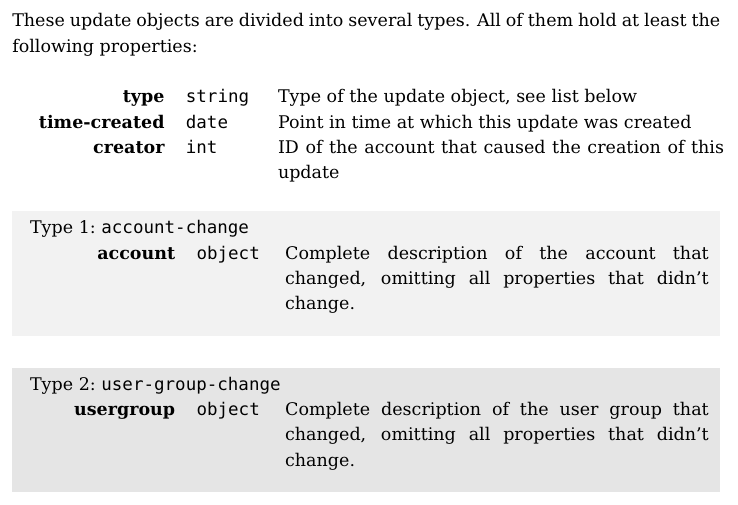
\includegraphics[width=1\textwidth]{images/Updates.png}
				\caption{Modellierung von Updates}
			\end{figure}
			\end{minipage}%
			\begin{minipage}{0.45\textwidth}
			\begin{itemize}
				\item[--] Updates als JsonObject dargestellt
				\item<2->[--] Befehle verursachen ggf. Updates für betroffene Klienten
				\item<3->[--] UpdateQueue für jeden Klienten
				\item<4->[--] Klient kann UpdateQueue per Befehl anfragen
				\item<5->[--] Server informiert Klienten über neue Updates

			\end{itemize}
			\end{minipage}
	\end{frame}

\end{document}
